% !TeX spellcheck = en_US
\documentclass{article}

% Pass options to natbib
\PassOptionsToPackage{numbers, compress}{natbib}

% NeurIPS packages
\usepackage[]{neurips_2023}
\usepackage[utf8]{inputenc} % allow utf-8 input
\usepackage[T1]{fontenc}    % use 8-bit T1 fonts
%\usepackage{hyperref}       % hyperlinks
\usepackage{url}            % simple URL typesetting
\usepackage{booktabs}       % professional-quality tables
\usepackage{amsfonts}       % blackboard math symbols
\usepackage{nicefrac}       % compact symbols for 1/2, etc.
\usepackage{microtype}      % microtypography
\usepackage{xcolor}         % colors

% Redefine paragraph to be tighter
\renewcommand{\paragraph}[1]{{\bf #1}~~}

% Array/table packages
\usepackage{tabularx}
\usepackage{array,multirow}
\usepackage{colortbl}
\newcommand{\PreserveBackslash}[1]{\let\temp=\\#1\let\\=\temp}
\newcolumntype{C}[1]{>{\PreserveBackslash\centering}p{#1}}
\newlength{\tblw}

% Latin
\usepackage{xspace}
\newcommand{\eg}{\textit{e.g.\@}\xspace}
\newcommand{\ie}{\textit{i.e.\@}\xspace}
\newcommand{\cf}{\textit{cf.\@}\xspace}
\newcommand{\etc}{\textit{etc.\@}\xspace}
\newcommand{\etal}{\textit{et~al.\@}\xspace}

% Our method
\newcommand{\our}{\textsc{sfr}\xspace}

% Tikz
\usepackage{tikz}
\usepackage{pgfplots}
\usetikzlibrary{patterns}
\usetikzlibrary{decorations,backgrounds,arrows.meta,calc}
\usetikzlibrary{shapes,arrows,positioning}

% Appendix/supplement title
\newcommand{\nipstitle}[1]{{%
    % rules for title box at top and bottom
    \def\toptitlebar{\hrule height4pt \vskip .25in \vskip -\parskip} 
    \def\bottomtitlebar{\vskip .29in \vskip -\parskip \hrule height1pt \vskip .09in} 
    \phantomsection\hsize\textwidth\linewidth\hsize%
    \vskip 0.1in%
    \toptitlebar%
    \begin{minipage}{\textwidth}%
        \centering{\LARGE\bf #1\par}%
    \end{minipage}%
    \bottomtitlebar%
    \addcontentsline{toc}{section}{#1}%
}}

% Bibliography
%\usepackage[maxcitenames=1, maxbibnames=4, doi=false, isbn=false, eprint=true, backend=bibtex, hyperref=true, url=false, style=authoryear-comp]{biblatex}
%\addbibresource{zotero-library.bib}
% \addbibresource{paper/zotero-library.bib}

% Let's use good old bibtex instead

% Figure customization: Tight legend box
\pgfplotsset{every axis/.append style={
		legend style={inner xsep=1pt, inner ysep=0.5pt, nodes={inner sep=1pt, text depth=0.1em},draw=none,fill=none}
}}

% Our packages
\usepackage{todonotes}
\usepackage[colorlinks=true,linkcolor=black,allcolors=black,urlcolor=black,citecolor=black]{hyperref}
\usepackage{amsmath}
\usepackage{bm}
\usepackage{algpseudocode}
\usepackage{algorithm}
\usepackage{derivative}
\usepackage{wrapfig}

\usepackage{tikz,pgfplots}
\usepackage{subcaption}
\usetikzlibrary{}

\newcommand{\defeq}{\vcentcolon=}

% Definitions/assumptions etc
\usepackage{mathtools}
\newtheorem{definition}{Definition}[section]
\newtheorem{assumption}{Assumption}[section]
\newtheorem{theorem}{Theorem}[section]
\newtheorem{lemma}{Lemma}[section]
% \newtheorem*{remark}{Remark}

% Short commands for commonly used stuff
\DeclareMathOperator{\R}{\mathbb{R}}
\DeclareMathOperator{\E}{\mathbb{E}}
\DeclareMathOperator{\V}{\mathbb{V}}


% Short section names etc
% This must be imported last!
%\usepackage{cleveref}
\usepackage[capitalise,nameinlink]{cleveref}
\crefname{section}{Sec.}{Secs.}
\crefname{algorithm}{Alg.}{Algs.}
\crefname{appendix}{App.}{Apps.}
\crefname{definition}{Def.}{Defs.}
\crefname{table}{Table}{Tables}

% Config for Arno's awesome TikZ plotting stuff
\newlength{\figurewidth}
\newlength{\figureheight}


% Variables
\newcommand{\state}{\ensuremath{\mathbf{s}}}
\newcommand{\action}{\ensuremath{\mathbf{a}}}
\newcommand{\noise}{\ensuremath{\bm\epsilon}}
\newcommand{\discount}{\ensuremath{\gamma}}
\newcommand{\inducingInput}{\ensuremath{\mathbf{Z}}}
\newcommand{\inducingVariable}{\ensuremath{\mathbf{u}}}
\newcommand{\dataset}{\ensuremath{\mathcal{D}}}
\newcommand{\dualParam}[1]{\ensuremath{\bm{\lambda}_{#1}}}
\newcommand{\meanParam}[1]{\ensuremath{\bm{\mu}_{#1}}}

% Indexes
\newcommand{\horizon}{\ensuremath{h}}
\newcommand{\Horizon}{\ensuremath{H}}
\newcommand{\numDataNew}{\ensuremath{N^{\text{new}}}}
\newcommand{\numDataOld}{\ensuremath{N^{\text{old}}}}
\newcommand{\numInducing}{\ensuremath{M}}

% Domains
\newcommand{\stateDomain}{\ensuremath{\mathcal{S}}}
\newcommand{\actionDomain}{\ensuremath{\mathcal{A}}}
\newcommand{\inputDomain}{\ensuremath{\mathbb{R}^{D}}}
\newcommand{\outputDomain}{\ensuremath{\mathbb{R}^{C}}}
\newcommand{\policyDomain}{\ensuremath{\Pi}}

% Functions
\newcommand{\rewardFn}{\ensuremath{r}}
\newcommand{\transitionFn}{\ensuremath{f}}
\newcommand{\latentFn}{\ensuremath{f}}

\newcommand{\optimisticTransition}{\ensuremath{\hat{f}}}
\newcommand{\optimisticTransitionMean}{\ensuremath{\mu_{\optimisticTransition}}}
\newcommand{\optimisticTransitionCov}{\ensuremath{\mu_{\optimisticTransition}}}
\newcommand{\optimisticTransitionSet}{\ensuremath{\mathcal{M}}}


% Parameters
% \newcommand{\weights}{\ensuremath{\bm\phi}}
\newcommand{\weights}{\ensuremath{\mathbf{w}}}
\newcommand{\valueFnParams}{\ensuremath{\psi}}
\newcommand{\policyParams}{\ensuremath{\theta}}

% Networks
\newcommand{\transitionFnWithParams}{\ensuremath{\transitionFn_{\weights}}}
\newcommand{\valueFn}{\ensuremath{\mathbf{Q}}}
\newcommand{\stateValueFn}{\ensuremath{\mathbf{V}}}
% \newcommand{\valueFn}{\ensuremath{\mathbf{Q}_{\valueFnParams}}}
\newcommand{\policy}{\ensuremath{\pi}}
\newcommand{\pPolicy}{\ensuremath{\pi_{\policyParams}}}


% Packages for bold math
\usepackage{bm}
\newcommand{\mathbold}[1]{\bm{#1}}
\newcommand{\mbf}[1]{\mathbf{#1}}
\renewcommand{\mid}{\,|\,}


% Math Macros
\newcommand{\MB}{\mbf{B}}
\newcommand{\MC}{\mbf{C}}
\newcommand{\MZ}{\mbf{Z}}
\newcommand{\MV}{\mbf{V}}
\newcommand{\MX}{\mbf{X}}
\newcommand{\MA}{\mbf{A}}
\newcommand{\MK}{\mbf{K}}
\newcommand{\MI}{\mbf{I}}
\newcommand{\MH}{\mbf{H}}
\newcommand{\T}{\top}
\newcommand{\vzeros}{\mbf{0}}
\newcommand{\vtheta}[0]{\mathbold{\theta}}
\newcommand{\valpha}[0]{\mathbold{\alpha}}
\newcommand{\vkappa}[0]{\mathbold{\kappa}}
\newcommand{\vbeta}[0]{\mathbold{\beta}}
\newcommand{\MBeta}[0]{\mathbold{B}}
\newcommand{\vlambda}[0]{\mathbold{\lambda}}
\newcommand{\diag}{\text{{diag}}}

\newcommand{\vm}{\mbf{m}}
\newcommand{\vz}{\mbf{z}}
\newcommand{\vf}{\mbf{f}}
\newcommand{\vu}{\mbf{u}}
\newcommand{\vx}{\mbf{x}}
\newcommand{\vy}{\mbf{y}}
\newcommand{\vw}{\mbf{w}}
\newcommand{\va}{\mbf{a}}

\newcommand{\Jac}[2]{\mathcal{J}_{#1}(#2)}
\newcommand{\JacT}[2]{\mathcal{J}_{#1}^\top(#2)}


\newcommand{\GP}{\mathcal{GP}}
\newcommand{\KL}[2]{\mathrm{D}_\textrm{KL} \dbar*{#1}{#2}}
\newcommand{\MKzz}{\mbf{K}_{\mbf{z}\mbf{z}}}
\newcommand{\MKzzc}{\mbf{K}_{\mbf{z}\mbf{z}, c}}
\newcommand{\MKxx}{\mbf{K}_{\mbf{x}\mbf{x}}}
\newcommand{\MKzx}{\mbf{K}_{\mbf{z}\mbf{x}}}
\newcommand{\MKxz}{\mbf{K}_{\mbf{x}\mbf{z}}}
\newcommand{\vkzi}{\mbf{k}_{\mbf{z}i}}
\newcommand{\vkzic}{\mbf{k}_{\mbf{z}i,c}}
\newcommand{\vkzs}{\mbf{k}_{\mbf{z}i}}
\newcommand{\vk}{\mbf{k}}
\newcommand{\MLambda}[0]{\mathbold{\Lambda}}
\newcommand{\MSigma}[0]{\mathbold{\Sigma}}
\definecolor{matplotlib-blue}{HTML}{1f77b4}
\newcommand{\N}{\mathrm{N}}
%\newcommand{\R}{\mathrm{R}}
\newcommand{\myexpect}{\mathbb{E}}

\DeclareMathOperator*{\argmax}{arg\,max}
\DeclareMathOperator*{\argmin}{arg\,min}
\newcommand{\Norm}{\mathcal{N}}

\newcommand{\digit}[1]{\tikz[baseline=-.5ex]\node[inner sep=1pt,rounded corners=1pt,draw=black,text width=5pt,minimum width=5pt,align=center,fill=black!20]{\tiny\bf\sf#1};}


%\title{Investigatin Uncertainty Quantification in Model-based Reinforcement Learning}
% \title{Model-based Reinforcement Learning with Fast Posterior Updates}
%\title{Sequential Decision-Making under Uncertainty with Big Data}
% \title{Neural Network to Vatiational Sparse Gaussian Process: For Adaptive Exploration}
% \title{Neural Network to Sparse Variational Gaussian Process: For Updates in Sequential Decision Making}
% \title{Adapting Neural Networks to New Data For Updates in Sequential Decision Making via Gaussian Processes}
% \title{Converting Neural Networks to Gaussian Processes for Sequential Decision-Making Under Uncertainty}
%\title{Sparse Function Space Representation of Neural Networks for Exploration and Retention}
%\title{Sparse Function-space Neural Networks}
% \title{Sparse Function-space Representation \\ of Neural Networks}% for Adaptation and Retention}
% \title{Rebuttal}% for Adaptation and Retention}
% \author{}


\begin{document}

% \maketitle

\begin{figure}[t]
  \centering\scriptsize
  \setlength{\figurewidth}{.26\textwidth}
  \setlength{\figureheight}{\figurewidth}
  \pgfplotsset{axis on top,scale only axis,y tick label style={rotate=90}, x tick label style={font=\footnotesize},y tick label style={font=\footnotesize},title style={yshift=-4pt,font=\large}, y label style={font=\large},x label style={font=\large},grid=major, width=\figurewidth, height=\figureheight}
  \pgfplotsset{grid style={line width=.1pt, draw=gray!10,dashed}}
  \pgfplotsset{xlabel={$M$},ylabel style={yshift=-12pt}}
  %
  \begin{minipage}[t]{.17\textwidth}
    \raggedleft
    \pgfplotsset{ylabel=NLPD}
    % This file was created by tikzplotlib v0.9.8.
\begin{tikzpicture}[scale=0.5]

\definecolor{color0}{rgb}{0.274509803921569,0.509803921568627,0.705882352941177}
\definecolor{color1}{rgb}{1,0.549019607843137,0}

\begin{axis}[
height=\figureheight,
tick align=outside,
tick pos=left,
title={\sc{Australian}},
width=\figurewidth,
x grid style={white!69.0196078431373!black},
xmin=-5, xmax=105,
xtick style={color=black},
xtick={-20,0,20,40,60,80,100,120},
xticklabels={\ensuremath{-}20,0,20,40,60,80,100,120},
y grid style={white!69.0196078431373!black},
ymin=0.293618057042495, ymax=0.718102694333381,
ytick style={color=black},
ytick={0.2,0.4,0.6,0.8},
yticklabels={0.2,0.4,0.6,0.8}
]
\path [draw=color0, fill=color0, opacity=0.1]
(axis cs:1,0.551667007775037)
--(axis cs:1,0.394871369856918)
--(axis cs:2,0.356818089006717)
--(axis cs:5,0.325282883209023)
--(axis cs:10,0.315017116932386)
--(axis cs:15,0.318190775561941)
--(axis cs:20,0.315173436351568)
--(axis cs:40,0.316824771925122)
--(axis cs:60,0.313980751125033)
--(axis cs:80,0.312912813282989)
--(axis cs:100,0.315163904006588)
--(axis cs:100,0.387714527539309)
--(axis cs:100,0.387714527539309)
--(axis cs:80,0.391337690954981)
--(axis cs:60,0.38348557249058)
--(axis cs:40,0.385913440494826)
--(axis cs:20,0.38626921460719)
--(axis cs:15,0.384456222562076)
--(axis cs:10,0.384020394527795)
--(axis cs:5,0.384817186909285)
--(axis cs:2,0.422463140257074)
--(axis cs:1,0.551667007775037)
--cycle;

\path [draw=color1, fill=color1, opacity=0.1]
(axis cs:1,0.698807938092886)
--(axis cs:1,0.662510632062247)
--(axis cs:2,0.657078817702754)
--(axis cs:5,0.517882131251046)
--(axis cs:10,0.40135987267536)
--(axis cs:15,0.393191142351973)
--(axis cs:20,0.371626166919784)
--(axis cs:40,0.35299934681048)
--(axis cs:60,0.324006125784774)
--(axis cs:80,0.327733599897042)
--(axis cs:100,0.315157958626014)
--(axis cs:100,0.388343247321801)
--(axis cs:100,0.388343247321801)
--(axis cs:80,0.39632234172613)
--(axis cs:60,0.39462009153726)
--(axis cs:40,0.403204497924365)
--(axis cs:20,0.453648844608426)
--(axis cs:15,0.468843614804632)
--(axis cs:10,0.622775822605122)
--(axis cs:5,0.646032048907283)
--(axis cs:2,0.691617433808421)
--(axis cs:1,0.698807938092886)
--cycle;

\addplot [semithick, color0]
table {%
1 0.473269188815977
2 0.389640614631896
5 0.355050035059154
10 0.349518755730091
15 0.351323499062008
20 0.350721325479379
40 0.351369106209974
60 0.348733161807807
80 0.352125252118985
100 0.351439215772948
};
\addplot [semithick, color1]
table {%
1 0.680659285077567
2 0.674348125755587
5 0.581957090079165
10 0.512067847640241
15 0.431017378578302
20 0.412637505764105
40 0.378101922367423
60 0.359313108661017
80 0.362027970811586
100 0.351750602973907
};
\end{axis}

\end{tikzpicture}

  \end{minipage}
  \hfill
%  \begin{minipage}[t]{.16\textwidth}
%    \raggedleft
%    % This file was created with tikzplotlib v0.10.1.
\begin{tikzpicture}

\definecolor{crimson2143940}{RGB}{214,39,40}
\definecolor{darkgray176}{RGB}{176,176,176}
\definecolor{darkorange25512714}{RGB}{255,127,14}
\definecolor{forestgreen4416044}{RGB}{44,160,44}
\definecolor{steelblue31119180}{RGB}{31,119,180}

\begin{axis}[
tick align=outside,
tick pos=left,
title={breast_cancer},
x grid style={darkgray176},
xlabel={Inducing points},
xmin=4, xmax=268,
xtick style={color=black},
xtick={0,50,100,150,200,250,300},
xticklabels={0,16,32,64,128,256,},
y grid style={darkgray176},
ylabel={Test NLPD},
ymin=0.0771, ymax=0.4929,
ytick style={color=black}
]
\addplot [semithick, steelblue31119180]
table {%
16 0.113
32 0.113
64 0.113
128 0.113
256 0.113
};
\addplot [semithick, darkorange25512714]
table {%
16 0.096
32 0.096
64 0.096
128 0.096
256 0.097
};
\addplot [semithick, forestgreen4416044]
table {%
16 0.474
32 0.409
64 0.289
128 0.201
256 0.141
};
\addplot [semithick, crimson2143940]
table {%
16 0.11
32 0.109
64 0.107
128 0.104
256 0.099
};
\end{axis}

\end{tikzpicture}

%  \end{minipage}
%  \hfill
%  \begin{minipage}[t]{.16\textwidth}
%    \raggedleft
%    % This file was created by tikzplotlib v0.9.8.
\begin{tikzpicture}[scale=0.5]

\definecolor{color0}{rgb}{0.274509803921569,0.509803921568627,0.705882352941177}
\definecolor{color1}{rgb}{1,0.549019607843137,0}

\begin{axis}[
height=\figureheight,
tick align=outside,
tick pos=left,
title={\sc{Ionosphere}},
width=\figurewidth,
x grid style={white!69.0196078431373!black},
xmin=-5, xmax=105,
xtick style={color=black},
xtick={-20,0,20,40,60,80,100,120},
xticklabels={\ensuremath{-}20,0,20,40,60,80,100,120},
y grid style={white!69.0196078431373!black},
ymin=0.318626138566577, ymax=0.739271476021987,
ytick style={color=black},
ytick={0.2,0.4,0.6,0.8},
yticklabels={0.2,0.4,0.6,0.8}
]
\path [draw=color0, fill=color0, opacity=0.1]
(axis cs:1,0.497740078146688)
--(axis cs:1,0.437140677802532)
--(axis cs:2,0.379856087932526)
--(axis cs:5,0.357508905697248)
--(axis cs:10,0.355612888961116)
--(axis cs:15,0.350074955147471)
--(axis cs:20,0.350186280222401)
--(axis cs:40,0.343992328389501)
--(axis cs:60,0.345364793630147)
--(axis cs:80,0.343065678108)
--(axis cs:100,0.344628619416667)
--(axis cs:100,0.458932033833142)
--(axis cs:100,0.458932033833142)
--(axis cs:80,0.458918417678441)
--(axis cs:60,0.421400983157666)
--(axis cs:40,0.426348073517958)
--(axis cs:20,0.421053565405504)
--(axis cs:15,0.420875168631528)
--(axis cs:10,0.421150947293654)
--(axis cs:5,0.427983327732078)
--(axis cs:2,0.480728220327442)
--(axis cs:1,0.497740078146688)
--cycle;

\path [draw=color1, fill=color1, opacity=0.1]
(axis cs:1,0.706539330239121)
--(axis cs:1,0.663164240747643)
--(axis cs:2,0.654018191556476)
--(axis cs:5,0.572564661558205)
--(axis cs:10,0.47167918260709)
--(axis cs:15,0.44288742819203)
--(axis cs:20,0.411502717536515)
--(axis cs:40,0.379578247364963)
--(axis cs:60,0.348844210695555)
--(axis cs:80,0.345346566039512)
--(axis cs:100,0.337746381178186)
--(axis cs:100,0.420668649757586)
--(axis cs:100,0.420668649757586)
--(axis cs:80,0.423796094341302)
--(axis cs:60,0.46841670929234)
--(axis cs:40,0.44232329846926)
--(axis cs:20,0.472082695977601)
--(axis cs:15,0.475740705754167)
--(axis cs:10,0.635139426788841)
--(axis cs:5,0.681819050687567)
--(axis cs:2,0.720151233410377)
--(axis cs:1,0.706539330239121)
--cycle;

\addplot [semithick, color0]
table {%
1 0.46744037797461
2 0.430292154129984
5 0.392746116714663
10 0.388381918127385
15 0.385475061889499
20 0.385619922813953
40 0.385170200953729
60 0.383382888393907
80 0.40099204789322
100 0.401780326624904
};
\addplot [semithick, color1]
table {%
1 0.684851785493382
2 0.687084712483427
5 0.627191856122886
10 0.553409304697965
15 0.459314066973099
20 0.441792706757058
40 0.410950772917112
60 0.408630459993947
80 0.384571330190407
100 0.379207515467886
};
\end{axis}

\end{tikzpicture}

%  \end{minipage}
%  \hfill
  \begin{minipage}[t]{.16\textwidth}
    \raggedleft
    % This file was created by tikzplotlib v0.9.8.
\begin{tikzpicture}[scale=0.5]

\definecolor{color0}{rgb}{0.274509803921569,0.509803921568627,0.705882352941177}
\definecolor{color1}{rgb}{1,0.549019607843137,0}

\begin{axis}[
height=\figureheight,
tick align=outside,
tick pos=left,
title={\sc{Glass}},
width=\figurewidth,
x grid style={white!69.0196078431373!black},
xmin=-5, xmax=105,
xtick style={color=black},
xtick={-20,0,20,40,60,80,100,120},
xticklabels={\ensuremath{-}20,0,20,40,60,80,100,120},
y grid style={white!69.0196078431373!black},
ymin=0.645730930143993, ymax=1.81802513016566,
ytick style={color=black}
]
\path [draw=color0, fill=color0, opacity=0.1]
(axis cs:1,1.49771547138196)
--(axis cs:1,1.18952652316133)
--(axis cs:1,1.18266373930492)
--(axis cs:5,0.96605549198983)
--(axis cs:9,0.857698870422498)
--(axis cs:15,0.78946981593607)
--(axis cs:19,0.809266568098092)
--(axis cs:39,0.762809039558936)
--(axis cs:59,0.699017030144978)
--(axis cs:79,0.729237532733376)
--(axis cs:99,0.720662924824656)
--(axis cs:99,1.04896167752313)
--(axis cs:99,1.04896167752313)
--(axis cs:79,0.995374423453727)
--(axis cs:59,1.0311643117542)
--(axis cs:39,1.02993831156299)
--(axis cs:19,1.03639284358281)
--(axis cs:15,1.04105346761967)
--(axis cs:9,1.02568275842161)
--(axis cs:5,1.16679810278829)
--(axis cs:1,1.35410828283228)
--(axis cs:1,1.49771547138196)
--cycle;

\path [draw=color1, fill=color1, opacity=0.1]
(axis cs:1,1.76473903016467)
--(axis cs:1,1.58753965664686)
--(axis cs:1,1.57139842233233)
--(axis cs:5,1.35246612424739)
--(axis cs:9,1.24713571688454)
--(axis cs:15,1.14321333399575)
--(axis cs:19,1.11838605334277)
--(axis cs:39,0.956363946082652)
--(axis cs:59,0.843593507041992)
--(axis cs:79,0.782856534900766)
--(axis cs:99,0.743711704977892)
--(axis cs:99,1.01490281645003)
--(axis cs:99,1.01490281645003)
--(axis cs:79,1.04688512529527)
--(axis cs:59,1.08499783743299)
--(axis cs:39,1.12512608223656)
--(axis cs:19,1.27061408651308)
--(axis cs:15,1.26826043220348)
--(axis cs:9,1.56711712146726)
--(axis cs:5,1.55216843320769)
--(axis cs:1,1.6887418957198)
--(axis cs:1,1.76473903016467)
--cycle;

\addplot [semithick, color0]
table {%
1 1.34362099727164
1 1.2683860110686
5 1.06642679738906
9 0.941690814422055
15 0.915261641777871
19 0.922829705840453
39 0.896373675560965
59 0.865090670949587
79 0.862305978093552
99 0.884812301173894
};
\addplot [semithick, color1]
table {%
1 1.67613934340577
1 1.63007015902607
5 1.45231727872754
9 1.4071264191759
15 1.20573688309961
19 1.19450006992792
39 1.0407450141596
59 0.96429567223749
79 0.914870830098019
99 0.879307260713959
};
\end{axis}

\end{tikzpicture}

  \end{minipage}
  \hfill
  \begin{minipage}[t]{.16\textwidth}
    \raggedleft
    % This file was created by tikzplotlib v0.9.8.
\begin{tikzpicture}

\definecolor{color0}{rgb}{0.274509803921569,0.509803921568627,0.705882352941177}
\definecolor{color1}{rgb}{1,0.549019607843137,0}

\begin{axis}[
height=\figureheight,
tick align=outside,
tick pos=left,
width=\figurewidth,
x grid style={white!69.0196078431373!black},
xlabel={\(\displaystyle M\) as \% of N},
xmin=-5, xmax=105,
xtick style={color=black},
xtick={-20,0,20,40,60,80,100,120},
xticklabels={\ensuremath{-}20,0,20,40,60,80,100,120},
y grid style={white!69.0196078431373!black},
ylabel={NLPD},
ymin=0.34357672797304, ymax=1.41475900431155,
ytick style={color=black}
]
\path [draw=color0, fill=color0, opacity=0.1]
(axis cs:1,1.241783829078)
--(axis cs:1,0.946697994349395)
--(axis cs:2,0.571557097293069)
--(axis cs:5,0.431461893359059)
--(axis cs:10,0.427250335376864)
--(axis cs:15,0.415079766983415)
--(axis cs:20,0.410897185776505)
--(axis cs:40,0.392266831442972)
--(axis cs:60,0.410732857158404)
--(axis cs:80,0.413736865021607)
--(axis cs:100,0.398539543245577)
--(axis cs:100,0.469322465409638)
--(axis cs:100,0.469322465409638)
--(axis cs:80,0.475593508085937)
--(axis cs:60,0.465626768932125)
--(axis cs:40,0.457891814856743)
--(axis cs:20,0.464778166479772)
--(axis cs:15,0.474885942468629)
--(axis cs:10,0.464577368596297)
--(axis cs:5,0.49541311907986)
--(axis cs:2,0.672678207688652)
--(axis cs:1,1.241783829078)
--cycle;

\path [draw=color1, fill=color1, opacity=0.1]
(axis cs:1,1.36606890084162)
--(axis cs:1,1.21439134599829)
--(axis cs:2,1.0817116290163)
--(axis cs:5,0.902314783290216)
--(axis cs:10,0.715655295957949)
--(axis cs:15,0.646190567422411)
--(axis cs:20,0.672836075045466)
--(axis cs:40,0.447776370520105)
--(axis cs:60,0.460253119410899)
--(axis cs:80,0.423214912886851)
--(axis cs:100,0.405288759175991)
--(axis cs:100,0.473603191580064)
--(axis cs:100,0.473603191580064)
--(axis cs:80,0.510302384047045)
--(axis cs:60,0.518577850665628)
--(axis cs:40,0.592697376377158)
--(axis cs:20,0.730283969675427)
--(axis cs:15,0.733130390245623)
--(axis cs:10,0.820111507096506)
--(axis cs:5,1.07747670080695)
--(axis cs:2,1.36423448550325)
--(axis cs:1,1.36606890084162)
--cycle;

\addplot [semithick, color0]
table {%
1 1.0942409117137
2 0.622117652490861
5 0.46343750621946
10 0.445913851986581
15 0.444982854726022
20 0.437837676128139
40 0.425079323149858
60 0.438179813045265
80 0.444665186553772
100 0.433931004327607
};
\addplot [semithick, color1]
table {%
1 1.29023012341995
2 1.22297305725977
5 0.989895742048583
10 0.767883401527228
15 0.689660478834017
20 0.701560022360446
40 0.520236873448632
60 0.489415485038263
80 0.466758648466948
100 0.439445975378028
};
\end{axis}

\end{tikzpicture}

  \end{minipage}
  \hfill
  \begin{minipage}[t]{.16\textwidth}
    \raggedleft
    % This file was created with tikzplotlib v0.10.1.
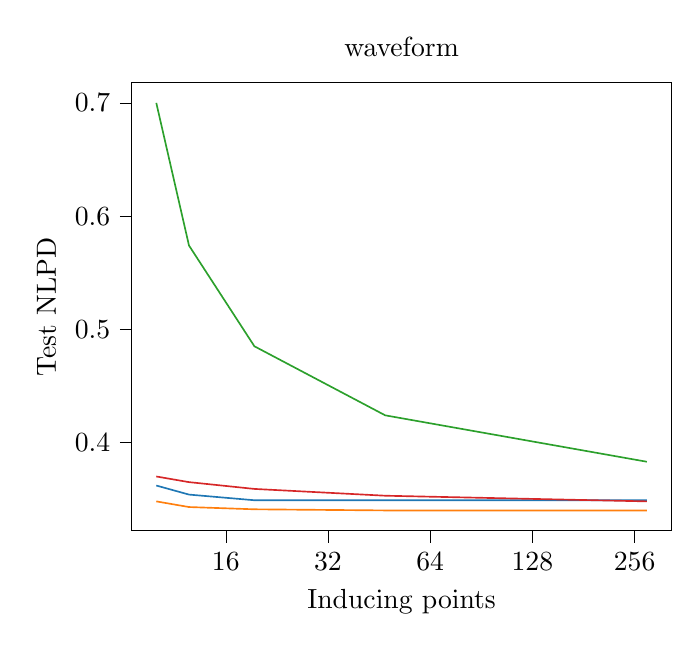
\begin{tikzpicture}

\definecolor{crimson2143940}{RGB}{214,39,40}
\definecolor{darkgray176}{RGB}{176,176,176}
\definecolor{darkorange25512714}{RGB}{255,127,14}
\definecolor{forestgreen4416044}{RGB}{44,160,44}
\definecolor{steelblue31119180}{RGB}{31,119,180}

\begin{axis}[
tick align=outside,
tick pos=left,
title={waveform},
x grid style={darkgray176},
xlabel={Inducing points},
xmin=4, xmax=268,
xtick style={color=black},
xtick={0,50,100,150,200,250,300},
xticklabels={0,16,32,64,128,256,},
y grid style={darkgray176},
ylabel={Test NLPD},
ymin=0.322, ymax=0.718,
ytick style={color=black}
]
\addplot [semithick, steelblue31119180]
table {%
16 0.362
32 0.354
64 0.349
128 0.349
256 0.349
};
\addplot [semithick, darkorange25512714]
table {%
16 0.348
32 0.343
64 0.341
128 0.34
256 0.34
};
\addplot [semithick, forestgreen4416044]
table {%
16 0.7
32 0.574
64 0.485
128 0.424
256 0.383
};
\addplot [semithick, crimson2143940]
table {%
16 0.37
32 0.365
64 0.359
128 0.353
256 0.348
};
\end{axis}

\end{tikzpicture}

  \end{minipage}
  \hfill
  \begin{minipage}[t]{.16\textwidth}
    \raggedleft
    % This file was created with tikzplotlib v0.10.1.
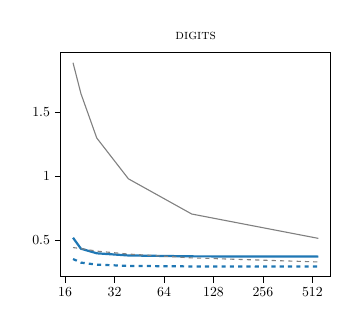
\begin{tikzpicture}[
scale=0.5
]

\definecolor{darkgray176}{RGB}{176,176,176}
\definecolor{gray}{RGB}{128,128,128}
\definecolor{steelblue31119180}{RGB}{31,119,180}

\begin{axis}[
tick align=outside,
tick pos=left,
title={\sc digits},
x grid style={darkgray176},
xmin=-8.8, xmax=536.8,
xtick style={color=black},
xtick={-100,0,100,200,300,400,500,600},
xticklabels={0,16,32,64,128,256,512,},
y grid style={darkgray176},
ymin=0.2101, ymax=1.9679,
ytick style={color=black}
]
\addplot [ultra thick, steelblue31119180]
table {%
16 0.516
32 0.43
64 0.394
128 0.377
256 0.37
512 0.368
};
\addplot [ultra thick, steelblue31119180, dashed]
table {%
16 0.349
32 0.321
64 0.305
128 0.295
256 0.291
512 0.29
};
\addplot [thick, gray]
table {%
16 1.888
32 1.646
64 1.298
128 0.978
256 0.702
512 0.511
};
\addplot [thick, gray, dashed]
table {%
16 0.439
32 0.431
64 0.411
128 0.388
256 0.358
512 0.326
};
\end{axis}

\end{tikzpicture}

  \end{minipage}
  \hfill
  \begin{minipage}[t]{.16\textwidth}
    \raggedleft
    % This file was created by tikzplotlib v0.9.8.
\begin{tikzpicture}

\definecolor{color0}{rgb}{0.274509803921569,0.509803921568627,0.705882352941177}
\definecolor{color1}{rgb}{1,0.549019607843137,0}

\begin{axis}[
height=\figureheight,
tick align=outside,
tick pos=left,
width=\figurewidth,
x grid style={white!69.0196078431373!black},
xlabel={\(\displaystyle M\) as \% of N},
xmin=-5, xmax=105,
xtick style={color=black},
xtick={-20,0,20,40,60,80,100,120},
xticklabels={\ensuremath{-}20,0,20,40,60,80,100,120},
y grid style={white!69.0196078431373!black},
ylabel={NLPD},
ymin=0.232868945885827, ymax=0.952205739288815,
ytick style={color=black},
ytick={0.2,0.4,0.6,0.8,1},
yticklabels={0.2,0.4,0.6,0.8,1.0}
]
\path [draw=color0, fill=color0, opacity=0.1]
(axis cs:1,0.391152761417344)
--(axis cs:1,0.321521954149105)
--(axis cs:2,0.282454703370333)
--(axis cs:5,0.294202713923217)
--(axis cs:10,0.26556607285869)
--(axis cs:15,0.2714883934195)
--(axis cs:20,0.267172403120068)
--(axis cs:40,0.2680998965525)
--(axis cs:60,0.268580750911881)
--(axis cs:60,0.31129434947327)
--(axis cs:60,0.31129434947327)
--(axis cs:40,0.337115320962889)
--(axis cs:20,0.345848237713317)
--(axis cs:15,0.326824039373233)
--(axis cs:10,0.331755020348582)
--(axis cs:5,0.342226542750507)
--(axis cs:2,0.346915562303046)
--(axis cs:1,0.391152761417344)
--cycle;

\path [draw=color1, fill=color1, opacity=0.1]
(axis cs:1,0.919508612315951)
--(axis cs:1,0.821918984692462)
--(axis cs:2,0.677101151550207)
--(axis cs:5,0.524269764776493)
--(axis cs:10,0.418282523447695)
--(axis cs:15,0.383338814008808)
--(axis cs:20,0.375641757595403)
--(axis cs:40,0.315946155255256)
--(axis cs:40,0.370004004383582)
--(axis cs:40,0.370004004383582)
--(axis cs:20,0.427686550442204)
--(axis cs:15,0.431995243421999)
--(axis cs:10,0.507855760482352)
--(axis cs:5,0.670933925464013)
--(axis cs:2,0.765602703537218)
--(axis cs:1,0.919508612315951)
--cycle;

\addplot [semithick, color0]
table {%
1 0.356337357783224
2 0.31468513283669
5 0.318214628336862
10 0.298660546603636
15 0.299156216396366
20 0.306510320416692
40 0.302607608757695
60 0.289937550192575
};
\addplot [semithick, color1]
table {%
1 0.870713798504207
2 0.721351927543713
5 0.597601845120253
10 0.463069141965024
15 0.407667028715403
20 0.401664154018804
40 0.342975079819419
};
\end{axis}

\end{tikzpicture}

  \end{minipage}\\[-1em]
  %
  % Legend
  \definecolor{steelblue31119180}{RGB}{31,119,180}
  \definecolor{darkorange25512714}{RGB}{255,127,14}
  \newcommand{\myline}[1]{\protect\tikz[baseline=-.5ex,line width=1.6pt]\protect\draw[draw=#1](0,0)--(1.2em,0);}
  \caption{Comparison of convergence in terms of number of inducing points $M$ in NLPD (mean over 10 seeds) on UCI classification tasks: \our (thick) vs.\ subsets (\cite{immer2021improving}, thin). Orange lines (\myline{darkorange25512714}) use the GP mean, whereas blue lines (\myline{steelblue31119180}) the NN MAP estimate as mean. Our \our converges fast for all cases.\looseness-1}
  \label{fig:uci-old}
  %\vspace*{-6pt}
\end{figure}

%
\begin{figure}[t]
  \centering\scriptsize
  \setlength{\figurewidth}{.26\textwidth}
  \setlength{\figureheight}{\figurewidth}
  \pgfplotsset{axis on top,scale only axis,y tick label style={rotate=90}, x tick label style={font=\footnotesize},y tick label style={font=\footnotesize},title style={yshift=-4pt,font=\large}, y label style={font=\large},x label style={font=\large},grid=major, width=\figurewidth, height=\figureheight}
  % \pgfplotsset{axis on top,scale only axis,y tick label style={rotate=90}, x tick label style={font=\footnotesize},y tick label style={font=\footnotesize},title style={yshift=-4pt,font=\large}, y label style={font=\large},x label style={font=\large},grid=major, width=\figurewidth, height=\figureheight}
  \pgfplotsset{grid style={line width=.1pt, draw=gray!10,dashed}}
  % \pgfplotsset{xlabel={$M$},ylabel style={yshift=-12pt}}
  %
  \begin{minipage}[t]{.1\textwidth}
    \raggedleft
    \pgfplotsset{ylabel=NLPD}
    % This file was created by tikzplotlib v0.9.8.
\begin{tikzpicture}[scale=0.5]

\definecolor{color0}{rgb}{0.274509803921569,0.509803921568627,0.705882352941177}
\definecolor{color1}{rgb}{1,0.549019607843137,0}

\begin{axis}[
height=\figureheight,
tick align=outside,
tick pos=left,
title={\sc{Australian}},
width=\figurewidth,
x grid style={white!69.0196078431373!black},
xmin=-5, xmax=105,
xtick style={color=black},
xtick={-20,0,20,40,60,80,100,120},
xticklabels={\ensuremath{-}20,0,20,40,60,80,100,120},
y grid style={white!69.0196078431373!black},
ymin=0.293618057042495, ymax=0.718102694333381,
ytick style={color=black},
ytick={0.2,0.4,0.6,0.8},
yticklabels={0.2,0.4,0.6,0.8}
]
\path [draw=color0, fill=color0, opacity=0.1]
(axis cs:1,0.551667007775037)
--(axis cs:1,0.394871369856918)
--(axis cs:2,0.356818089006717)
--(axis cs:5,0.325282883209023)
--(axis cs:10,0.315017116932386)
--(axis cs:15,0.318190775561941)
--(axis cs:20,0.315173436351568)
--(axis cs:40,0.316824771925122)
--(axis cs:60,0.313980751125033)
--(axis cs:80,0.312912813282989)
--(axis cs:100,0.315163904006588)
--(axis cs:100,0.387714527539309)
--(axis cs:100,0.387714527539309)
--(axis cs:80,0.391337690954981)
--(axis cs:60,0.38348557249058)
--(axis cs:40,0.385913440494826)
--(axis cs:20,0.38626921460719)
--(axis cs:15,0.384456222562076)
--(axis cs:10,0.384020394527795)
--(axis cs:5,0.384817186909285)
--(axis cs:2,0.422463140257074)
--(axis cs:1,0.551667007775037)
--cycle;

\path [draw=color1, fill=color1, opacity=0.1]
(axis cs:1,0.698807938092886)
--(axis cs:1,0.662510632062247)
--(axis cs:2,0.657078817702754)
--(axis cs:5,0.517882131251046)
--(axis cs:10,0.40135987267536)
--(axis cs:15,0.393191142351973)
--(axis cs:20,0.371626166919784)
--(axis cs:40,0.35299934681048)
--(axis cs:60,0.324006125784774)
--(axis cs:80,0.327733599897042)
--(axis cs:100,0.315157958626014)
--(axis cs:100,0.388343247321801)
--(axis cs:100,0.388343247321801)
--(axis cs:80,0.39632234172613)
--(axis cs:60,0.39462009153726)
--(axis cs:40,0.403204497924365)
--(axis cs:20,0.453648844608426)
--(axis cs:15,0.468843614804632)
--(axis cs:10,0.622775822605122)
--(axis cs:5,0.646032048907283)
--(axis cs:2,0.691617433808421)
--(axis cs:1,0.698807938092886)
--cycle;

\addplot [semithick, color0]
table {%
1 0.473269188815977
2 0.389640614631896
5 0.355050035059154
10 0.349518755730091
15 0.351323499062008
20 0.350721325479379
40 0.351369106209974
60 0.348733161807807
80 0.352125252118985
100 0.351439215772948
};
\addplot [semithick, color1]
table {%
1 0.680659285077567
2 0.674348125755587
5 0.581957090079165
10 0.512067847640241
15 0.431017378578302
20 0.412637505764105
40 0.378101922367423
60 0.359313108661017
80 0.362027970811586
100 0.351750602973907
};
\end{axis}

\end{tikzpicture}

  \end{minipage}
  \hfill
%  \begin{minipage}[t]{.16\textwidth}
%    \raggedleft
%    % This file was created with tikzplotlib v0.10.1.
\begin{tikzpicture}

\definecolor{crimson2143940}{RGB}{214,39,40}
\definecolor{darkgray176}{RGB}{176,176,176}
\definecolor{darkorange25512714}{RGB}{255,127,14}
\definecolor{forestgreen4416044}{RGB}{44,160,44}
\definecolor{steelblue31119180}{RGB}{31,119,180}

\begin{axis}[
tick align=outside,
tick pos=left,
title={breast_cancer},
x grid style={darkgray176},
xlabel={Inducing points},
xmin=4, xmax=268,
xtick style={color=black},
xtick={0,50,100,150,200,250,300},
xticklabels={0,16,32,64,128,256,},
y grid style={darkgray176},
ylabel={Test NLPD},
ymin=0.0771, ymax=0.4929,
ytick style={color=black}
]
\addplot [semithick, steelblue31119180]
table {%
16 0.113
32 0.113
64 0.113
128 0.113
256 0.113
};
\addplot [semithick, darkorange25512714]
table {%
16 0.096
32 0.096
64 0.096
128 0.096
256 0.097
};
\addplot [semithick, forestgreen4416044]
table {%
16 0.474
32 0.409
64 0.289
128 0.201
256 0.141
};
\addplot [semithick, crimson2143940]
table {%
16 0.11
32 0.109
64 0.107
128 0.104
256 0.099
};
\end{axis}

\end{tikzpicture}

%  \end{minipage}
%  \hfill
%  \begin{minipage}[t]{.16\textwidth}
%    \raggedleft
%    % This file was created by tikzplotlib v0.9.8.
\begin{tikzpicture}[scale=0.5]

\definecolor{color0}{rgb}{0.274509803921569,0.509803921568627,0.705882352941177}
\definecolor{color1}{rgb}{1,0.549019607843137,0}

\begin{axis}[
height=\figureheight,
tick align=outside,
tick pos=left,
title={\sc{Ionosphere}},
width=\figurewidth,
x grid style={white!69.0196078431373!black},
xmin=-5, xmax=105,
xtick style={color=black},
xtick={-20,0,20,40,60,80,100,120},
xticklabels={\ensuremath{-}20,0,20,40,60,80,100,120},
y grid style={white!69.0196078431373!black},
ymin=0.318626138566577, ymax=0.739271476021987,
ytick style={color=black},
ytick={0.2,0.4,0.6,0.8},
yticklabels={0.2,0.4,0.6,0.8}
]
\path [draw=color0, fill=color0, opacity=0.1]
(axis cs:1,0.497740078146688)
--(axis cs:1,0.437140677802532)
--(axis cs:2,0.379856087932526)
--(axis cs:5,0.357508905697248)
--(axis cs:10,0.355612888961116)
--(axis cs:15,0.350074955147471)
--(axis cs:20,0.350186280222401)
--(axis cs:40,0.343992328389501)
--(axis cs:60,0.345364793630147)
--(axis cs:80,0.343065678108)
--(axis cs:100,0.344628619416667)
--(axis cs:100,0.458932033833142)
--(axis cs:100,0.458932033833142)
--(axis cs:80,0.458918417678441)
--(axis cs:60,0.421400983157666)
--(axis cs:40,0.426348073517958)
--(axis cs:20,0.421053565405504)
--(axis cs:15,0.420875168631528)
--(axis cs:10,0.421150947293654)
--(axis cs:5,0.427983327732078)
--(axis cs:2,0.480728220327442)
--(axis cs:1,0.497740078146688)
--cycle;

\path [draw=color1, fill=color1, opacity=0.1]
(axis cs:1,0.706539330239121)
--(axis cs:1,0.663164240747643)
--(axis cs:2,0.654018191556476)
--(axis cs:5,0.572564661558205)
--(axis cs:10,0.47167918260709)
--(axis cs:15,0.44288742819203)
--(axis cs:20,0.411502717536515)
--(axis cs:40,0.379578247364963)
--(axis cs:60,0.348844210695555)
--(axis cs:80,0.345346566039512)
--(axis cs:100,0.337746381178186)
--(axis cs:100,0.420668649757586)
--(axis cs:100,0.420668649757586)
--(axis cs:80,0.423796094341302)
--(axis cs:60,0.46841670929234)
--(axis cs:40,0.44232329846926)
--(axis cs:20,0.472082695977601)
--(axis cs:15,0.475740705754167)
--(axis cs:10,0.635139426788841)
--(axis cs:5,0.681819050687567)
--(axis cs:2,0.720151233410377)
--(axis cs:1,0.706539330239121)
--cycle;

\addplot [semithick, color0]
table {%
1 0.46744037797461
2 0.430292154129984
5 0.392746116714663
10 0.388381918127385
15 0.385475061889499
20 0.385619922813953
40 0.385170200953729
60 0.383382888393907
80 0.40099204789322
100 0.401780326624904
};
\addplot [semithick, color1]
table {%
1 0.684851785493382
2 0.687084712483427
5 0.627191856122886
10 0.553409304697965
15 0.459314066973099
20 0.441792706757058
40 0.410950772917112
60 0.408630459993947
80 0.384571330190407
100 0.379207515467886
};
\end{axis}

\end{tikzpicture}

%  \end{minipage}
%  \hfill
  \begin{minipage}[t]{.1\textwidth}
    \raggedleft
    % This file was created by tikzplotlib v0.9.8.
\begin{tikzpicture}[scale=0.5]

\definecolor{color0}{rgb}{0.274509803921569,0.509803921568627,0.705882352941177}
\definecolor{color1}{rgb}{1,0.549019607843137,0}

\begin{axis}[
height=\figureheight,
tick align=outside,
tick pos=left,
title={\sc{Glass}},
width=\figurewidth,
x grid style={white!69.0196078431373!black},
xmin=-5, xmax=105,
xtick style={color=black},
xtick={-20,0,20,40,60,80,100,120},
xticklabels={\ensuremath{-}20,0,20,40,60,80,100,120},
y grid style={white!69.0196078431373!black},
ymin=0.645730930143993, ymax=1.81802513016566,
ytick style={color=black}
]
\path [draw=color0, fill=color0, opacity=0.1]
(axis cs:1,1.49771547138196)
--(axis cs:1,1.18952652316133)
--(axis cs:1,1.18266373930492)
--(axis cs:5,0.96605549198983)
--(axis cs:9,0.857698870422498)
--(axis cs:15,0.78946981593607)
--(axis cs:19,0.809266568098092)
--(axis cs:39,0.762809039558936)
--(axis cs:59,0.699017030144978)
--(axis cs:79,0.729237532733376)
--(axis cs:99,0.720662924824656)
--(axis cs:99,1.04896167752313)
--(axis cs:99,1.04896167752313)
--(axis cs:79,0.995374423453727)
--(axis cs:59,1.0311643117542)
--(axis cs:39,1.02993831156299)
--(axis cs:19,1.03639284358281)
--(axis cs:15,1.04105346761967)
--(axis cs:9,1.02568275842161)
--(axis cs:5,1.16679810278829)
--(axis cs:1,1.35410828283228)
--(axis cs:1,1.49771547138196)
--cycle;

\path [draw=color1, fill=color1, opacity=0.1]
(axis cs:1,1.76473903016467)
--(axis cs:1,1.58753965664686)
--(axis cs:1,1.57139842233233)
--(axis cs:5,1.35246612424739)
--(axis cs:9,1.24713571688454)
--(axis cs:15,1.14321333399575)
--(axis cs:19,1.11838605334277)
--(axis cs:39,0.956363946082652)
--(axis cs:59,0.843593507041992)
--(axis cs:79,0.782856534900766)
--(axis cs:99,0.743711704977892)
--(axis cs:99,1.01490281645003)
--(axis cs:99,1.01490281645003)
--(axis cs:79,1.04688512529527)
--(axis cs:59,1.08499783743299)
--(axis cs:39,1.12512608223656)
--(axis cs:19,1.27061408651308)
--(axis cs:15,1.26826043220348)
--(axis cs:9,1.56711712146726)
--(axis cs:5,1.55216843320769)
--(axis cs:1,1.6887418957198)
--(axis cs:1,1.76473903016467)
--cycle;

\addplot [semithick, color0]
table {%
1 1.34362099727164
1 1.2683860110686
5 1.06642679738906
9 0.941690814422055
15 0.915261641777871
19 0.922829705840453
39 0.896373675560965
59 0.865090670949587
79 0.862305978093552
99 0.884812301173894
};
\addplot [semithick, color1]
table {%
1 1.67613934340577
1 1.63007015902607
5 1.45231727872754
9 1.4071264191759
15 1.20573688309961
19 1.19450006992792
39 1.0407450141596
59 0.96429567223749
79 0.914870830098019
99 0.879307260713959
};
\end{axis}

\end{tikzpicture}

  \end{minipage}
  \hfill
  \begin{minipage}[t]{.1\textwidth}
    \raggedleft
    % This file was created by tikzplotlib v0.9.8.
\begin{tikzpicture}

\definecolor{color0}{rgb}{0.274509803921569,0.509803921568627,0.705882352941177}
\definecolor{color1}{rgb}{1,0.549019607843137,0}

\begin{axis}[
height=\figureheight,
tick align=outside,
tick pos=left,
width=\figurewidth,
x grid style={white!69.0196078431373!black},
xlabel={\(\displaystyle M\) as \% of N},
xmin=-5, xmax=105,
xtick style={color=black},
xtick={-20,0,20,40,60,80,100,120},
xticklabels={\ensuremath{-}20,0,20,40,60,80,100,120},
y grid style={white!69.0196078431373!black},
ylabel={NLPD},
ymin=0.34357672797304, ymax=1.41475900431155,
ytick style={color=black}
]
\path [draw=color0, fill=color0, opacity=0.1]
(axis cs:1,1.241783829078)
--(axis cs:1,0.946697994349395)
--(axis cs:2,0.571557097293069)
--(axis cs:5,0.431461893359059)
--(axis cs:10,0.427250335376864)
--(axis cs:15,0.415079766983415)
--(axis cs:20,0.410897185776505)
--(axis cs:40,0.392266831442972)
--(axis cs:60,0.410732857158404)
--(axis cs:80,0.413736865021607)
--(axis cs:100,0.398539543245577)
--(axis cs:100,0.469322465409638)
--(axis cs:100,0.469322465409638)
--(axis cs:80,0.475593508085937)
--(axis cs:60,0.465626768932125)
--(axis cs:40,0.457891814856743)
--(axis cs:20,0.464778166479772)
--(axis cs:15,0.474885942468629)
--(axis cs:10,0.464577368596297)
--(axis cs:5,0.49541311907986)
--(axis cs:2,0.672678207688652)
--(axis cs:1,1.241783829078)
--cycle;

\path [draw=color1, fill=color1, opacity=0.1]
(axis cs:1,1.36606890084162)
--(axis cs:1,1.21439134599829)
--(axis cs:2,1.0817116290163)
--(axis cs:5,0.902314783290216)
--(axis cs:10,0.715655295957949)
--(axis cs:15,0.646190567422411)
--(axis cs:20,0.672836075045466)
--(axis cs:40,0.447776370520105)
--(axis cs:60,0.460253119410899)
--(axis cs:80,0.423214912886851)
--(axis cs:100,0.405288759175991)
--(axis cs:100,0.473603191580064)
--(axis cs:100,0.473603191580064)
--(axis cs:80,0.510302384047045)
--(axis cs:60,0.518577850665628)
--(axis cs:40,0.592697376377158)
--(axis cs:20,0.730283969675427)
--(axis cs:15,0.733130390245623)
--(axis cs:10,0.820111507096506)
--(axis cs:5,1.07747670080695)
--(axis cs:2,1.36423448550325)
--(axis cs:1,1.36606890084162)
--cycle;

\addplot [semithick, color0]
table {%
1 1.0942409117137
2 0.622117652490861
5 0.46343750621946
10 0.445913851986581
15 0.444982854726022
20 0.437837676128139
40 0.425079323149858
60 0.438179813045265
80 0.444665186553772
100 0.433931004327607
};
\addplot [semithick, color1]
table {%
1 1.29023012341995
2 1.22297305725977
5 0.989895742048583
10 0.767883401527228
15 0.689660478834017
20 0.701560022360446
40 0.520236873448632
60 0.489415485038263
80 0.466758648466948
100 0.439445975378028
};
\end{axis}

\end{tikzpicture}

  \end{minipage}
  \hfill
  \begin{minipage}[t]{.1\textwidth}
    \raggedleft
    % This file was created with tikzplotlib v0.10.1.
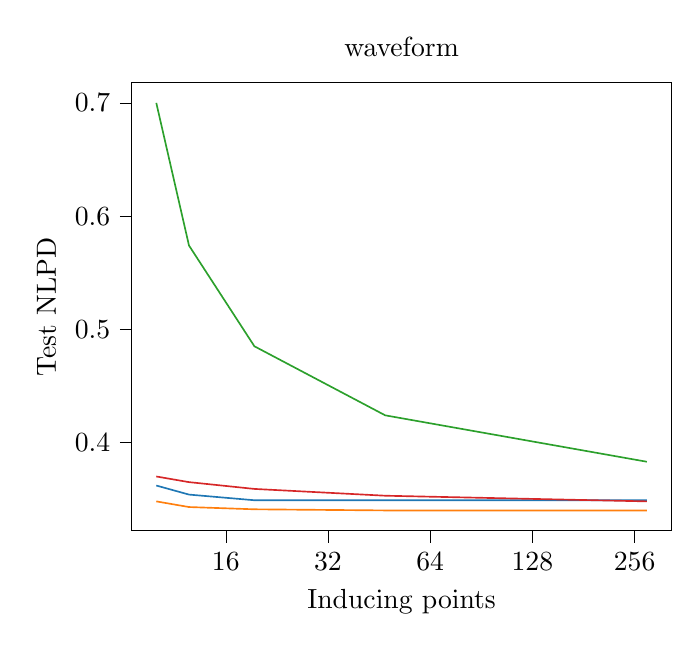
\begin{tikzpicture}

\definecolor{crimson2143940}{RGB}{214,39,40}
\definecolor{darkgray176}{RGB}{176,176,176}
\definecolor{darkorange25512714}{RGB}{255,127,14}
\definecolor{forestgreen4416044}{RGB}{44,160,44}
\definecolor{steelblue31119180}{RGB}{31,119,180}

\begin{axis}[
tick align=outside,
tick pos=left,
title={waveform},
x grid style={darkgray176},
xlabel={Inducing points},
xmin=4, xmax=268,
xtick style={color=black},
xtick={0,50,100,150,200,250,300},
xticklabels={0,16,32,64,128,256,},
y grid style={darkgray176},
ylabel={Test NLPD},
ymin=0.322, ymax=0.718,
ytick style={color=black}
]
\addplot [semithick, steelblue31119180]
table {%
16 0.362
32 0.354
64 0.349
128 0.349
256 0.349
};
\addplot [semithick, darkorange25512714]
table {%
16 0.348
32 0.343
64 0.341
128 0.34
256 0.34
};
\addplot [semithick, forestgreen4416044]
table {%
16 0.7
32 0.574
64 0.485
128 0.424
256 0.383
};
\addplot [semithick, crimson2143940]
table {%
16 0.37
32 0.365
64 0.359
128 0.353
256 0.348
};
\end{axis}

\end{tikzpicture}

  \end{minipage}
  \hfill
  \begin{minipage}[t]{.1\textwidth}
    \raggedleft
    % This file was created with tikzplotlib v0.10.1.
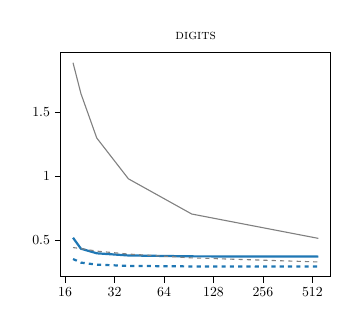
\begin{tikzpicture}[
scale=0.5
]

\definecolor{darkgray176}{RGB}{176,176,176}
\definecolor{gray}{RGB}{128,128,128}
\definecolor{steelblue31119180}{RGB}{31,119,180}

\begin{axis}[
tick align=outside,
tick pos=left,
title={\sc digits},
x grid style={darkgray176},
xmin=-8.8, xmax=536.8,
xtick style={color=black},
xtick={-100,0,100,200,300,400,500,600},
xticklabels={0,16,32,64,128,256,512,},
y grid style={darkgray176},
ymin=0.2101, ymax=1.9679,
ytick style={color=black}
]
\addplot [ultra thick, steelblue31119180]
table {%
16 0.516
32 0.43
64 0.394
128 0.377
256 0.37
512 0.368
};
\addplot [ultra thick, steelblue31119180, dashed]
table {%
16 0.349
32 0.321
64 0.305
128 0.295
256 0.291
512 0.29
};
\addplot [thick, gray]
table {%
16 1.888
32 1.646
64 1.298
128 0.978
256 0.702
512 0.511
};
\addplot [thick, gray, dashed]
table {%
16 0.439
32 0.431
64 0.411
128 0.388
256 0.358
512 0.326
};
\end{axis}

\end{tikzpicture}

  \end{minipage}
  \hfill
  \begin{minipage}[t]{.1\textwidth}
    \raggedleft
    % This file was created by tikzplotlib v0.9.8.
\begin{tikzpicture}

\definecolor{color0}{rgb}{0.274509803921569,0.509803921568627,0.705882352941177}
\definecolor{color1}{rgb}{1,0.549019607843137,0}

\begin{axis}[
height=\figureheight,
tick align=outside,
tick pos=left,
width=\figurewidth,
x grid style={white!69.0196078431373!black},
xlabel={\(\displaystyle M\) as \% of N},
xmin=-5, xmax=105,
xtick style={color=black},
xtick={-20,0,20,40,60,80,100,120},
xticklabels={\ensuremath{-}20,0,20,40,60,80,100,120},
y grid style={white!69.0196078431373!black},
ylabel={NLPD},
ymin=0.232868945885827, ymax=0.952205739288815,
ytick style={color=black},
ytick={0.2,0.4,0.6,0.8,1},
yticklabels={0.2,0.4,0.6,0.8,1.0}
]
\path [draw=color0, fill=color0, opacity=0.1]
(axis cs:1,0.391152761417344)
--(axis cs:1,0.321521954149105)
--(axis cs:2,0.282454703370333)
--(axis cs:5,0.294202713923217)
--(axis cs:10,0.26556607285869)
--(axis cs:15,0.2714883934195)
--(axis cs:20,0.267172403120068)
--(axis cs:40,0.2680998965525)
--(axis cs:60,0.268580750911881)
--(axis cs:60,0.31129434947327)
--(axis cs:60,0.31129434947327)
--(axis cs:40,0.337115320962889)
--(axis cs:20,0.345848237713317)
--(axis cs:15,0.326824039373233)
--(axis cs:10,0.331755020348582)
--(axis cs:5,0.342226542750507)
--(axis cs:2,0.346915562303046)
--(axis cs:1,0.391152761417344)
--cycle;

\path [draw=color1, fill=color1, opacity=0.1]
(axis cs:1,0.919508612315951)
--(axis cs:1,0.821918984692462)
--(axis cs:2,0.677101151550207)
--(axis cs:5,0.524269764776493)
--(axis cs:10,0.418282523447695)
--(axis cs:15,0.383338814008808)
--(axis cs:20,0.375641757595403)
--(axis cs:40,0.315946155255256)
--(axis cs:40,0.370004004383582)
--(axis cs:40,0.370004004383582)
--(axis cs:20,0.427686550442204)
--(axis cs:15,0.431995243421999)
--(axis cs:10,0.507855760482352)
--(axis cs:5,0.670933925464013)
--(axis cs:2,0.765602703537218)
--(axis cs:1,0.919508612315951)
--cycle;

\addplot [semithick, color0]
table {%
1 0.356337357783224
2 0.31468513283669
5 0.318214628336862
10 0.298660546603636
15 0.299156216396366
20 0.306510320416692
40 0.302607608757695
60 0.289937550192575
};
\addplot [semithick, color1]
table {%
1 0.870713798504207
2 0.721351927543713
5 0.597601845120253
10 0.463069141965024
15 0.407667028715403
20 0.401664154018804
40 0.342975079819419
};
\end{axis}

\end{tikzpicture}

  \end{minipage}\\[-1em]
  %
  % Legend
  \definecolor{steelblue31119180}{RGB}{31,119,180}
  \definecolor{darkorange25512714}{RGB}{255,127,14}
  \newcommand{\myline}[1]{\protect\tikz[baseline=-.5ex,line width=1.6pt]\protect\draw[draw=#1](0,0)--(1.2em,0);}
  \caption{Comparison of convergence in terms of number of inducing points $M$ in NLPD (mean over 10 seeds) on UCI classification tasks: \our (thick) vs.\ subsets (\cite{immer2021improving}, thin). Orange lines (\myline{darkorange25512714}) use the GP mean, whereas blue lines (\myline{steelblue31119180}) the NN MAP estimate as mean. Our \our converges fast for all cases.\looseness-1}
  \label{fig:uci}
  %\vspace*{-6pt}
\end{figure}

% \clearpage


% \phantomsection%
% \addcontentsline{toc}{section}{References}
% \begingroup
% \small
% \bibliographystyle{abbrvnat}
% \bibliography{bibliography}%zotero-library
% \endgroup

\end{document}
